\documentclass[11pt]{article}
\usepackage{amsmath}
\usepackage{amssymb}
\usepackage{amsthm}
\usepackage{amscd}
\usepackage{amsfonts}
\usepackage{graphicx}
\usepackage{color}
\usepackage{amsfonts}
\usepackage{amsthm}
\usepackage{psfrag} 
\usepackage{graphicx,url,newverbs}



\usepackage{amsfonts,verbatim}
\usepackage{amssymb}
\usepackage{amsmath}
\usepackage{subfigure}
\usepackage{psfrag,curves,algorithm2e}


\newcommand{\fig}[1]{\mbox{Figure{~#1}}}

\newcommand{\ubar}[1]{\text{\b{$#1$}}}

\usepackage[top=2.8cm,bottom=2.8cm,left=2.5cm,right=2.5cm]{geometry}
%===============================================================
%Fonts

\usepackage[default]{cantarell} %% Use option "defaultsans" to use cantarell as sans serif only
\usepackage[T1]{fontenc}

\usepackage[affil-it]{authblk} 
%\usepackage{lmodern}

%=============================================================



\newcommand{\ba}{\begin{array}}
\newcommand{\ea}{\end{array}}
\newcommand{\be}{\begin{equation}}
\newcommand{\ee}{\end{equation}}
\newcommand{\bd}{\begin{displaymath}}
\newcommand{\ed}{\end{displaymath}}
\newcommand{\pa}{\partial}
\newcommand{\f}{\frac}
\newcommand{\vh}{\hat{v}}
\newcommand{\uh}{\hat{u}}
\newcommand{\uhe}{{\hat{u}_1}}
\newcommand{\uht}{{\hat{u}_2}}
\newcommand{\calo}{{\cal O}}
\newcommand{\nb}{{\bf n}}

\newcommand{\dpx}{D_+}
\newcommand{\dmx}{D_-}


\usepackage[dvipsnames]{xcolor}
% \definecolor{mypink1}{rgb}{0.858, 0.188, 0.478}
% \definecolor{mypink2}{RGB}{219, 48, 122}
% \definecolor{mypink3}{cmyk}{0, 0.7808, 0.4429, 0.1412}
% \definecolor{mygray}{gray}{0.6}

\newcommand{\daniel}[1]{{{\color{black} {#1}}}}
\usepackage{newverbs}
\newverbcommand{\fortran}{\color{Aquamarine}}{}

\DeclareMathOperator*{\argmin}{arg\,min}

\begin{document}

\title{MTH Numerical PDE\\ Collaborative Project - Spring 2021}
\author{Daniel Appel{\"o}\thanks{appeloda@msu.edu}}
\affil{Department of Computational Mathematics, Science \& Engineering \\ 
Department of Mathematics, \\
Michigan State University, East Lansing MI 48824, USA.}
\date{\small \today}
\maketitle

\begin{center}
\setlength{\unitlength}{0.7cm} 
\begin{picture}(7,7) 
\qbezier(1,1)(3.5,0.5)(2,2)
\qbezier(2,2)(1.5,2.5)(1,2)
\qbezier(1,2)(0.2,1.2)(1,1)
\put(0.6,2.3){$\Gamma_1$} 

\qbezier(5,1)(5.9,1.3)(5,3)
\qbezier(5,3)(4,5)(4,2.2)
\qbezier(4,2.2)(4,1)(5,1)
\put(5.2,3.1){$\Gamma_2$} 


\qbezier(2,4)(1.3,5)(2,6)
\qbezier(2,6)(3.0,7.0)(3,5.5)
\qbezier(3,5.5)(3.1,1.8)(2,4)
\put(3.1,5.3){$\Gamma_3$} 

\qbezier(0.9,0.4)(4.5,0)(6.3,0.4)
\qbezier(6.3,0.4)(6.6,0.5)(6.6,0.7)
\qbezier(6.6,0.7)(7,4.5)(6.6,6.3)
\qbezier(6.6,6.3)(6.5,6.45)(6.3,6.5)
\qbezier(6.3,6.5)(4.5,7)(0.8,6.5)
\qbezier(0.8,6.5)(0.63,6.48)(0.5,6.2)
\qbezier(0.5,6.2)(0,4.5)(0.5,0.9)
\qbezier(0.5,0.9)(0.55,0.45)(0.9,0.4)

\put(6,6){$\Gamma_4$} 
\end{picture}
\hspace{0.5cm}
\begin{picture}(7,7) 
\multiput(0,0)(0,0.7){11}{\line(1,0){7}}
\multiput(0,0)(0.7,0){11}{\line(0,1){7}}

\qbezier(1,1)(3.5,0.5)(2,2)
\qbezier(2,2)(1.5,2.5)(1,2)
\qbezier(1,2)(0.2,1.2)(1,1)
\put(0.6,2.3){$\Gamma_1$} 

\qbezier(5,1)(5.9,1.3)(5,3)
\qbezier(5,3)(4,5)(4,2.2)
\qbezier(4,2.2)(4,1)(5,1)
\put(5.2,3.1){$\Gamma_2$} 


\qbezier(2,4)(1.3,5)(2,6)
\qbezier(2,6)(3.0,7.0)(3,5.5)
\qbezier(3,5.5)(3.1,1.8)(2,4)
\put(3.1,5.3){$\Gamma_3$} 

\qbezier(0.9,0.4)(4.5,0)(6.3,0.4)
\qbezier(6.3,0.4)(6.6,0.5)(6.6,0.7)
\qbezier(6.6,0.7)(7,4.5)(6.6,6.3)
\qbezier(6.6,6.3)(6.5,6.45)(6.3,6.5)
\qbezier(6.3,6.5)(4.5,7)(0.8,6.5)
\qbezier(0.8,6.5)(0.63,6.48)(0.5,6.2)
\qbezier(0.5,6.2)(0,4.5)(0.5,0.9)
\qbezier(0.5,0.9)(0.55,0.45)(0.9,0.4)

\put(6,6){$\Gamma_4$} 
\end{picture}
\hspace{0.5cm}
\begin{picture}(7,7) 
\multiput(0,0)(0,0.7){11}{\line(1,0){7}}
\multiput(0,0)(0.7,0){11}{\line(0,1){7}}

\multiput(0.7,0.7)(0.7,0){9}{\circle*{0.15}}
\multiput(2.8,1.4)(0.7,0){2}{\circle*{0.15}}
\multiput(5.6,1.4)(0.7,0){2}{\circle*{0.15}}
\multiput(0.7,2.1)(0.7,0){1}{\circle*{0.15}}
\multiput(2.1,2.1)(0.7,0){3}{\circle*{0.15}}
\multiput(5.6,2.1)(0.7,0){2}{\circle*{0.15}}
\multiput(0.7,2.8)(0.7,0){5}{\circle*{0.15}}
\multiput(5.6,2.8)(0.7,0){2}{\circle*{0.15}}
\multiput(0.7,3.5)(0.7,0){3}{\circle*{0.15}}
\multiput(3.5,3.5)(0.7,0){1}{\circle*{0.15}}
\multiput(4.9,3.5)(0.7,0){3}{\circle*{0.15}}
\multiput(0.7,4.2)(0.7,0){2}{\circle*{0.15}}
\multiput(3.5,4.2)(0.7,0){5}{\circle*{0.15}}
\multiput(0.7,4.9)(0.7,0){2}{\circle*{0.15}}
\multiput(3.5,4.9)(0.7,0){5}{\circle*{0.15}}
\multiput(0.7,5.6)(0.7,0){2}{\circle*{0.15}}
\multiput(3.5,5.6)(0.7,0){5}{\circle*{0.15}}
\multiput(0.7,6.3)(0.7,0){3}{\circle*{0.15}}
\multiput(3.5,6.3)(0.7,0){5}{\circle*{0.15}}

\qbezier(1,1)(3.5,0.5)(2,2)
\qbezier(2,2)(1.5,2.5)(1,2)
\qbezier(1,2)(0.2,1.2)(1,1)
\put(0.6,2.3){$\Gamma_1$} 

\qbezier(5,1)(5.9,1.3)(5,3)
\qbezier(5,3)(4,5)(4,2.2)
\qbezier(4,2.2)(4,1)(5,1)
\put(5.2,3.1){$\Gamma_2$} 

\qbezier(2,4)(1.3,5)(2,6)
\qbezier(2,6)(3.0,7.0)(3,5.5)
\qbezier(3,5.5)(3.1,1.8)(2,4)
\put(3.1,5.3){$\Gamma_3$} 

\qbezier(0.9,0.4)(4.5,0)(6.3,0.4)
\qbezier(6.3,0.4)(6.6,0.5)(6.6,0.7)
\qbezier(6.6,0.7)(7,4.5)(6.6,6.3)
\qbezier(6.6,6.3)(6.5,6.45)(6.3,6.5)
\qbezier(6.3,6.5)(4.5,7)(0.8,6.5)
\qbezier(0.8,6.5)(0.63,6.48)(0.5,6.2)
\qbezier(0.5,6.2)(0,4.5)(0.5,0.9)
\qbezier(0.5,0.9)(0.55,0.45)(0.9,0.4)

\put(6,6){$\Gamma_4$} 
\end{picture}
\end{center}

\vspace{1cm}
 \begin{center}
 \psfrag{x1}[][][0.9][0]{$x$}
 \psfrag{y1}[][][0.9][270]{$y$}
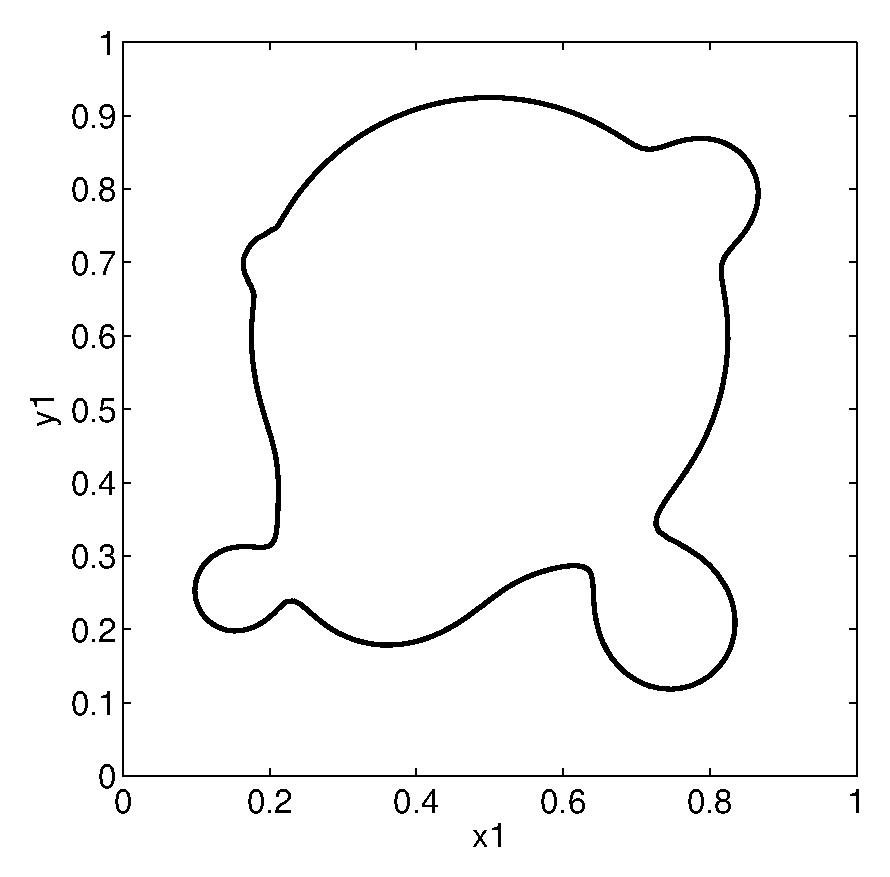
\includegraphics[width=0.3\textwidth]{Membrane}
\hspace{0.2cm}
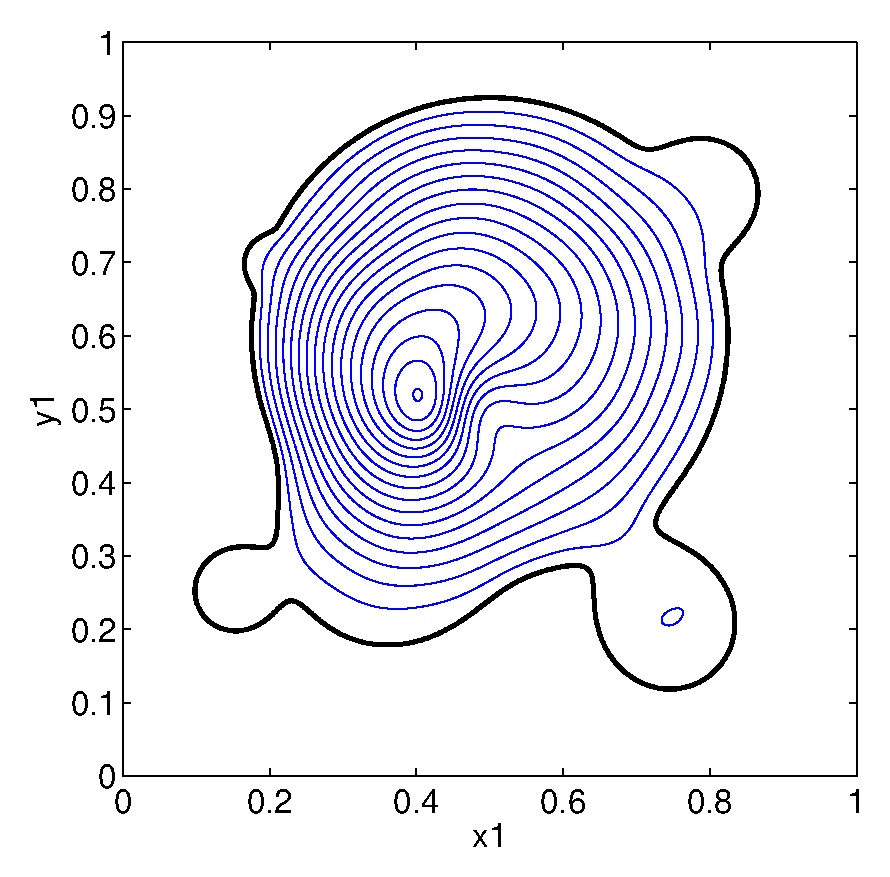
\includegraphics[width=0.3\textwidth]{Mode1}
\hspace{0.2cm}
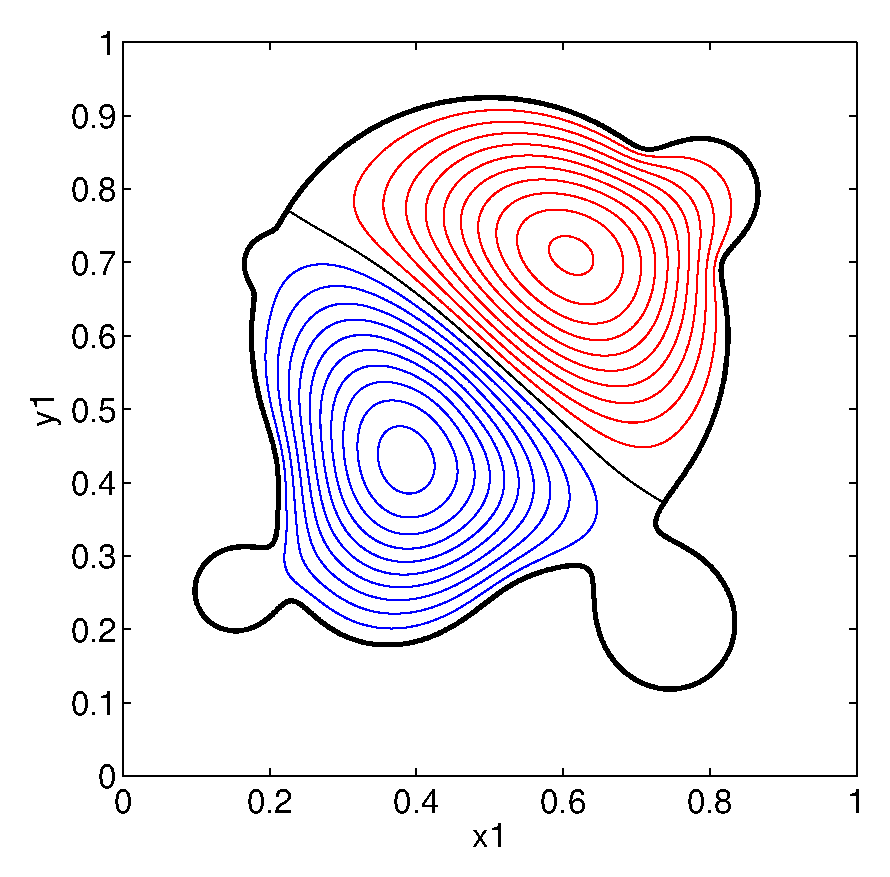
\includegraphics[width=0.3\textwidth]{Mode2}
\end{center}


\clearpage

\section{Introduction}
In this project we will implement a variation of the embedded boundary (EB) method proposed by Kreiss et al. in \cite{kreiss:1940}. The method in \cite{kreiss:1940} is designed to solve the scalar wave equation on a Cartesian grid with an embedded boundary representing  a complex geometry.  

We will only consider the case of Dirichlet boundary conditions here but the ideas can be generalized to other boundary conditions. Unlike the method in \cite{kreiss:1940} we will use my idea from \cite{AppPetEB09} to place the ``ghost-points'' on the inside of the computational domain rather than the outside. This simplifies the implementation a bit. 

The method we will implement consists of three distinct building blocks: 
\begin{enumerate}
\item boundary condition enforcement,
\item spatial discretization, 
\item and temporal discretization. 
\end{enumerate}
Each of these blocks can be modified independently of the others to suit a particular applications. For example, it would be straightforward to handle smoothly variable coefficients or mixed Neumann and Dirichlet boundary conditions. 

\section{Description of the method}\label{sec:descroption}
\begin{figure}[htb]
\begin{center}
\subfigure[Exterior problem.]{
\setlength{\unitlength}{0.7cm} 
\begin{picture}(7,7) 

\qbezier(1,1)(3.5,0.5)(2,2)
\qbezier(2,2)(1.5,2.5)(1,2)
\qbezier(1,2)(0.2,1.2)(1,1)
\put(0.6,2.3){$\Gamma_1$} 

\qbezier(5,1)(5.9,1.3)(5,3)
\qbezier(5,3)(4,5)(4,2.2)
\qbezier(4,2.2)(4,1)(5,1)
\put(5.2,3.1){$\Gamma_2$} 


\qbezier(2,4)(1.3,5)(2,6)
\qbezier(2,6)(3.0,7.0)(3,5.5)
\qbezier(3,5.5)(3.1,1.8)(2,4)
\put(3.1,5.3){$\Gamma_3$} 

\end{picture}
}
\subfigure[Interior problem.]{
\setlength{\unitlength}{0.7cm} 
\begin{picture}(7,7) 
\qbezier(1,1)(3.5,0.5)(2,2)
\qbezier(2,2)(1.5,2.5)(1,2)
\qbezier(1,2)(0.2,1.2)(1,1)
\put(0.6,2.3){$\Gamma_1$} 

\qbezier(5,1)(5.9,1.3)(5,3)
\qbezier(5,3)(4,5)(4,2.2)
\qbezier(4,2.2)(4,1)(5,1)
\put(5.2,3.1){$\Gamma_2$} 


\qbezier(2,4)(1.3,5)(2,6)
\qbezier(2,6)(3.0,7.0)(3,5.5)
\qbezier(3,5.5)(3.1,1.8)(2,4)
\put(3.1,5.3){$\Gamma_3$} 

\qbezier(0.9,0.4)(4.5,0)(6.3,0.4)
\qbezier(6.3,0.4)(6.6,0.5)(6.6,0.7)
\qbezier(6.6,0.7)(7,4.5)(6.6,6.3)
\qbezier(6.6,6.3)(6.5,6.45)(6.3,6.5)
\qbezier(6.3,6.5)(4.5,7)(0.8,6.5)
\qbezier(0.8,6.5)(0.63,6.48)(0.5,6.2)
\qbezier(0.5,6.2)(0,4.5)(0.5,0.9)
\qbezier(0.5,0.9)(0.55,0.45)(0.9,0.4)

\put(6,6){$\Gamma_4$} 
\end{picture}
}
\caption{Possible setups. Note that the setup (a) must be augmented by boundary conditions at infinity.\label{fig:probsetup}}
\end{center}
\end{figure}
We consider the wave equation in a two-dimensional domain $(x,y)\in\Omega$ in an isotropic medium
with a constant speed of sound (for simplicity set to one) 
%
\be \label{eq:weq} 
\f{\pa^2 u}{\pa t^2} =
\f{\pa^2 u}{\pa x^2} + \f{\pa^2 u}{\pa y^2} + f,\quad (x,y)\in\Omega,\ t\geq 0,
\ee 
%
with initial data 
%
\be \label{eq:weqid1} 
u(x,y,0) = g_0(x,y), \quad \f{\pa u}{\pa t}(x,y,0) = g_1(x,y), \quad (x,y)\in\Omega,
\ee 
%
and boundary conditions of Dirichlet type
%
\be
\label{eq:weqbcD} u(x,y,t) = h^{(i)}_{\mathcal{D}}(x,y,t),\quad (x,y)\in \Gamma_l, \ t\geq 0,\ l=1,\ldots, n_{\rm tot}. 
\ee 
The boundary of the simply connected domain $\Omega$ is a collection of $n_{\text{tot}}$ smooth
curves $\Gamma_l$. For an exterior problem the curves $\Gamma_l$ must be augmented by a boundary condition at
infinity or by a non-reflecting boundary condition. For an interior problem one curve encloses the
$n_{\rm tot}-1$ other curves, as shown in \fig{\ref{fig:probsetup}}.


\subsection{Pre-computations}\label{sec:Precomp}
\begin{figure}[htb]
\begin{center}
\subfigure[]{
\setlength{\unitlength}{0.7cm} 
\begin{picture}(7,7) 
\multiput(0,0)(0,0.7){11}{\line(1,0){7}}
\multiput(0,0)(0.7,0){11}{\line(0,1){7}}

\qbezier(1,1)(3.5,0.5)(2,2)
\qbezier(2,2)(1.5,2.5)(1,2)
\qbezier(1,2)(0.2,1.2)(1,1)
\put(0.6,2.3){$\Gamma_1$} 

\qbezier(5,1)(5.9,1.3)(5,3)
\qbezier(5,3)(4,5)(4,2.2)
\qbezier(4,2.2)(4,1)(5,1)
\put(5.2,3.1){$\Gamma_2$} 


\qbezier(2,4)(1.3,5)(2,6)
\qbezier(2,6)(3.0,7.0)(3,5.5)
\qbezier(3,5.5)(3.1,1.8)(2,4)
\put(3.1,5.3){$\Gamma_3$} 

\qbezier(0.9,0.4)(4.5,0)(6.3,0.4)
\qbezier(6.3,0.4)(6.6,0.5)(6.6,0.7)
\qbezier(6.6,0.7)(7,4.5)(6.6,6.3)
\qbezier(6.6,6.3)(6.5,6.45)(6.3,6.5)
\qbezier(6.3,6.5)(4.5,7)(0.8,6.5)
\qbezier(0.8,6.5)(0.63,6.48)(0.5,6.2)
\qbezier(0.5,6.2)(0,4.5)(0.5,0.9)
\qbezier(0.5,0.9)(0.55,0.45)(0.9,0.4)

\put(6,6){$\Gamma_4$} 
\end{picture}
}
\subfigure[]{
\setlength{\unitlength}{0.7cm} 
\begin{picture}(7,7) 
\multiput(0,0)(0,0.7){11}{\line(1,0){7}}
\multiput(0,0)(0.7,0){11}{\line(0,1){7}}

\multiput(0.7,0.7)(0.7,0){9}{\circle*{0.15}}
\multiput(2.8,1.4)(0.7,0){2}{\circle*{0.15}}
\multiput(5.6,1.4)(0.7,0){2}{\circle*{0.15}}
\multiput(0.7,2.1)(0.7,0){1}{\circle*{0.15}}
\multiput(2.1,2.1)(0.7,0){3}{\circle*{0.15}}
\multiput(5.6,2.1)(0.7,0){2}{\circle*{0.15}}
\multiput(0.7,2.8)(0.7,0){5}{\circle*{0.15}}
\multiput(5.6,2.8)(0.7,0){2}{\circle*{0.15}}
\multiput(0.7,3.5)(0.7,0){3}{\circle*{0.15}}
\multiput(3.5,3.5)(0.7,0){1}{\circle*{0.15}}
\multiput(4.9,3.5)(0.7,0){3}{\circle*{0.15}}
\multiput(0.7,4.2)(0.7,0){2}{\circle*{0.15}}
\multiput(3.5,4.2)(0.7,0){5}{\circle*{0.15}}
\multiput(0.7,4.9)(0.7,0){2}{\circle*{0.15}}
\multiput(3.5,4.9)(0.7,0){5}{\circle*{0.15}}
\multiput(0.7,5.6)(0.7,0){2}{\circle*{0.15}}
\multiput(3.5,5.6)(0.7,0){5}{\circle*{0.15}}
\multiput(0.7,6.3)(0.7,0){3}{\circle*{0.15}}
\multiput(3.5,6.3)(0.7,0){5}{\circle*{0.15}}

\qbezier(1,1)(3.5,0.5)(2,2)
\qbezier(2,2)(1.5,2.5)(1,2)
\qbezier(1,2)(0.2,1.2)(1,1)
\put(0.6,2.3){$\Gamma_1$} 

\qbezier(5,1)(5.9,1.3)(5,3)
\qbezier(5,3)(4,5)(4,2.2)
\qbezier(4,2.2)(4,1)(5,1)
\put(5.2,3.1){$\Gamma_2$} 

\qbezier(2,4)(1.3,5)(2,6)
\qbezier(2,6)(3.0,7.0)(3,5.5)
\qbezier(3,5.5)(3.1,1.8)(2,4)
\put(3.1,5.3){$\Gamma_3$} 

\qbezier(0.9,0.4)(4.5,0)(6.3,0.4)
\qbezier(6.3,0.4)(6.6,0.5)(6.6,0.7)
\qbezier(6.6,0.7)(7,4.5)(6.6,6.3)
\qbezier(6.6,6.3)(6.5,6.45)(6.3,6.5)
\qbezier(6.3,6.5)(4.5,7)(0.8,6.5)
\qbezier(0.8,6.5)(0.63,6.48)(0.5,6.2)
\qbezier(0.5,6.2)(0,4.5)(0.5,0.9)
\qbezier(0.5,0.9)(0.55,0.45)(0.9,0.4)

\put(6,6){$\Gamma_4$} 
\end{picture}
}
\caption{Discretization of the geometry without the mask shown (a) and with the mask shown (b), dots
indicate $m_{ij}=1$.\label{fig:probsetupdiscrete}}
\end{center}
\end{figure}
To find an approximate solution to equations (\ref{eq:weq})-(\ref{eq:weqbcD}) we assume, without
restriction, that all curves describing the geometry are contained inside a rectangular domain
$(x,y) \in \Omega = [0,L_x] \times [0,L_y]$ and cover $\Omega$ with the uniform grid (see
\fig{\ref{fig:probsetupdiscrete}})
%
\bd
(x_i,y_j) = ((i-1)h,(j-1)h),\ \ i=1,\ldots,n_x,\, j=1,\ldots,n_y.
\ed
%
\begin{itemize}
\item The grid size $h>0$ and the number of grid points are chosen such that $x_{n_x}=L_x$ and
$y_{n_y} = L_y$. 

\item We denote a time dependent grid function by $u_{ij}(t) = u(x_i,y_j,t)$. 
\item Time is discretized on a equidistant grid $t_n = n k$ with time-step $k>0$, and a time discrete
grid function is denoted $u^n_{ij} = u(x_i,y_j,t_n)$.
\end{itemize}
The solution to (\ref{eq:weq}) is sought only at grid points inside $\Omega$. In a
pre-computation step a mask grid function $m_{i,j}$ is set up such that
\[
m_{i,j} = \begin{cases}
1,&(x_i,y_j)\in\Omega,\\
0,&\mbox{otherwise}.
\end{cases}
\]
The mask is particularly easy to set up when the boundary of $\Omega$ is defined by the implicit
representation $\phi(x,y)$=0, a so called level-set function. In this case, $m_{i,j}$ simply follows by the sign of
$\phi(x_i,y_j)$.  An example of a mask grid function
is shown in \fig{\ref{fig:probsetupdiscrete}}.

Boundary conditions are enforced by assigning values to the grid points on the fringe of the
computational domain $\Omega$. These points are denoted \emph{boundary points}. 
\begin{itemize}
\item A \emph{boundary
point} $(x_p,y_q)$ is distinguished by the following criterion: $m_{p,q} = 1$ and $m_{p+1,q} +
m_{p-1,q} +m_{p,q+1} +m_{p,q-1} < 4$, i.e., the boundary point is inside $\Omega$, but at least one
of its nearest neighbors is outside. 
\item The \emph{boundary points} define $x$- and $y$-\emph{line
segments} upon which approximations to the spatial derivatives in (\ref{eq:weq}) are computed. For
example, an $x$-\emph{line segment} is defined as the collection of grid points $(x_{p},y_q),\, p =
p_1,\ldots,p_2$ with $m_{p,q}=1$, starting and ending at \emph{boundary points}, $(x_{p_1},y_q)$ and
$(x_{p_2},y_q)$, respectively. 
\item The \emph{boundary points} and the \emph{line segments} are found by inspecting the mask.
\end{itemize}

To find approximations to spatial derivatives at all points inside the computational domain it is
sufficient to know all \emph{line segments}. However, to also account for boundary conditions some
additional pre-computations must be performed to determine the stencil and coefficients in the
formula for assigning solution values at each \emph{boundary point}. The procedure for setting up
such \emph{boundary stencils} depends on the type of boundary conditions and the approach taken to
enforce them. For Dirichlet boundary conditions a one-dimensional line-by-line approach can be used
which is described in \S\ref{sec:linebyline}. The advantage of this approach is ease of
implementation. Other options are possible see \cite{AppPetEB09}.

\subsubsection{Enforcing Dirichlet boundary conditions along grid lines}\label{sec:linebyline}
Let $(x_i, y_j)$ be a \emph{boundary point} associated with a boundary $\Gamma_l$ where the solution is
prescribed. To assign a value to $u_{ij}$ we introduce a local one-dimensional coordinate system
$\xi$ along the grid line in $x$ passing through $(x_i,y_j)$ (left image of
\fig{\ref{fig:LinebylineD}}), and construct an interpolating polynomial 
%
\be \label{eq:Interpolant}
\mathcal{I}u(\xi) = u_{ij} g_{ij}(\xi) + u_{1} g_{1}(\xi).  
\ee 
%
Here $g_{ij}(\xi),\, g_1(\xi)$ are  polynomials in the usual Lagrange polynomial basis. Now, by equating the
interpolant evaluated on the boundary with the right hand side of the boundary condition 
%
\bd \mathcal{I}u(\xi_{\Gamma}) =
h_{\mathcal{D}}(x_\Gamma,y_{\Gamma},t), 
\ed
%
we obtain an explicit expression for $u_{ij}$ 
%
\be
\label{eq:DirichletLineByLine} u_{ij} = \frac{1}{g_{ij}(\xi_\Gamma)}
\left(h_{\mathcal{D}}(x_\Gamma,y_{\Gamma},t) -  u_{1}
g_{1}(\xi_\Gamma)\right).
\ee 
%
Note that once the intersection of the boundary, $\xi_\Gamma$, is found (e.g.~by using a
root-finding algorithm such as the secant method) the numbers $g_{ij}(\xi_\Gamma)$,
$g_{1}(\xi_\Gamma)$,  do not depend on time and can be pre-computed and
stored. 
\begin{figure}[htb]
\begin{center}
\setlength{\unitlength}{0.8cm} 
\begin{picture}(7,7) 
% Grid
\multiput(0,1)(0,1){2}{\line(1,0){7}}
\multiput(0,4)(0,1){3}{\line(1,0){7}}
\multiput(1,0)(1,0){6}{\line(0,1){7}}
% Curve
\qbezier(5.5,6.5)(-2.5,1.5)(4.8,0.2)
\put(2,3){\circle{0.25}}
\put(3,3){\circle*{0.25}}
%\put(4,3){\circle*{0.25}}
%\put(5,3){\circle*{0.25}}
%\put(6,3){\circle*{0.25}}

\put(2.05,3.2){$u_{ij}$} 
\put(3.05,3.2){$u_{1}$} 
%\put(4.05,3.2){$u_{2}$} 
%\put(5.05,3.2){$u_{3}$} 
%\put(6.05,3.2){$u_{4}$} 

\put(3.2,5.3){$\Gamma_l$}
\put(2.05,2.5){$\xi_{ij}$} 
\put(3.05,2.5){$\xi_{1}$} 
%\put(4.05,2.5){$\xi_{2}$} 
%\put(5.05,2.5){$\xi_{3}$} 
%\put(6.05,2.5){$\xi_{4}$} 

\put(2.45,1.5){$\xi_{\Gamma}$} 
\put(2.75,1.75){\vector(-1,1){1.2}}


\thicklines
\put(0.5,3){\vector(1,0){6.4}}
\put(6.8,2.5){$\xi$}
\end{picture}
\hspace{0.3cm}
\setlength{\unitlength}{0.8cm} 
\begin{picture}(7,7) 
% Grid
\multiput(0,1)(0,1){2}{\line(1,0){7}}
\multiput(0,4)(0,1){3}{\line(1,0){7}}
\multiput(1,0)(1,0){6}{\line(0,1){7}}
% Curve
\qbezier(5.5,6.5)(-2.5,1.5)(4.8,0.2)
\put(1,3){\circle{0.25}}
\put(2,3){\circle*{0.25}}
%\put(3,3){\circle*{0.25}}
%\put(4,3){\circle*{0.25}}
%\put(5,3){\circle*{0.25}}

\put(1.05,3.2){$u_{ij}$} 
\put(2.05,3.2){$u_{1}$} 
%\put(3.05,3.2){$u_{2}$} 
%\put(4.05,3.2){$u_{3}$} 
%\put(5.05,3.2){$u_{4}$} 

\put(0.35,2.5){$\xi_{ij}$} 
\put(2.05,2.5){$\xi_{1}$} 
%\put(3.05,2.5){$\xi_{2}$} 
%\put(4.05,2.5){$\xi_{3}$} 
%\put(5.05,2.5){$\xi_{4}$} 

\put(2.45,1.5){$\xi_{\Gamma}$} 
\put(2.75,1.75){\vector(-1,1){1.2}}

\put(3.2,5.3){$\Gamma_l$}

\thicklines
\put(0.5,3){\vector(1,0){6.4}}
\put(6.8,2.5){$\xi$}
\end{picture}
\caption{Enforcing Dirichlet boundary conditions by a line by line approach using interior {\em boundary
points} (left) or exterior {\em ghost points} (right).\label{fig:LinebylineD}}
\end{center}
\end{figure}

The placement of the \emph{boundary point} is the subtle yet important distinction from previous
methods like those in \cite{Kreiss_Petersson_2006,kreiss:1940,kreiss:1292}. In previous work the \emph{ghost point} is placed outside the
computational domain as pictured in the right image of \fig{\ref{fig:LinebylineD}}. This placement
has the disadvantage that the denominator of (\ref{eq:DirichletLineByLine}):
%
\bd
g_{ij}(\xi_\Gamma) = \f{\xi_\Gamma-\xi_{1}}{\xi_{ij}-\xi_{1}},
\ed
%
may become arbitrary small when $\xi_\Gamma$ is close to $\xi_{1}$ causing small-cell stiffness in
an explicit time stepping procedure.

In contrast, for the approach suggested above, $\xi_\Gamma \le \xi_{ij} < \xi_1 = \xi_{ij}+h$, and thus  
%
\bd
| \xi_\Gamma - \xi_1|  \ge | \xi_{ij} - \xi_1|  = h,
\ed  
%
so $g_{ij}(\xi_\Gamma)$ is always bounded away from zero. 

\subsection{One dimension and no embedded boundary}
In one dimension the scalar wave equation takes the form
%
\be \label{eq:weq1d} 
\f{\pa^2 u}{\pa t^2} =
\f{\pa^2 u}{\pa x^2} + f,\quad x \in [0,L_x],\ t\geq 0,
\ee 
%
with initial data 
%
\be \label{eq:weqid1d} 
u(x,0) = g_0(x), \quad \f{\pa u}{\pa t}(x,0) = g_1(x), \quad x \in [0,L_x],
\ee 
and with boundary conditions 
\be
u(0,t) = h_0(t), \ \ u(L_x,t) = h_1(t).
\ee

Here as the boundaries align with the first and last gridpoint we can easily write down a second order accurate approximation. The initial data for the displacement is
\[
u^0_{i} = g_0({x_i}),  i = 1,\ldots,n_x. 
\]
We then use the displacement and velocity initial conditions to approximate the solution at time $t = -k$. We have the Taylor expansion 
\[
	u(x,-k) \approx u(x,0) - k u_t(x,0) + \frac{k^2}{2} u_{tt}(x,0),
\]
which together with the equation gives 
\[
u^{-1}_{i} = g_0({x_i}) - k g_1({x_i}) +\frac{k^2}{2} \left( \dpx \dmx g_0(x_i)  + f(x_i,0) \right) ,  i = 2,\ldots,n_x-1. 
\]
The boundary conditions are
\[
u^n_{1} = h_0(t_n), \ \  u^n_{n_x} = h_1(t_n).
\]
Finally to discretize the equation we use centered finite differences in space and time and get the update formula
\be
u^{n+1}_i = 2u^n_i - u^{n-1}_i +k^2(\dpx \dmx u^n_i + f^n_i), \ \  i = 2,\ldots,n_x-1. 
\ee

{\bf Today we will see how to implement this.}






\section{Method of Manufactured Solution or Twilight Zone Forcing}
Say that we are interested in finding a discrete approximation, $v$, to the solution of the initial-boundary-value-problem 
\begin{align}
&u_{tt}=u_{xx}+f, \ \ t > 0,\, x\in[0,1], \label{pde}\\
& u(x,0) = u_0(x),\label{ic}\\
& \alpha_0 u(0,t) +\alpha_1 u_x(0,t) = u_l(t), \label{bc0}\\ 
& \beta_0 u(1,t) +\beta_1 u_x(1,t) = u_r(t), \label{bc1}
\end{align}
by implementing some numerical method on a computer. How can we convince ourselves (and the instructor or TA) that the code  is implementing the numerical method and thus approximating the ivbp correctly? 

Assume that the numerical method has an error that converges to zero with some discretization parameter $h$ (usually the grid spacing) as $\mathcal{O}(h^r)$. Then a good test is to measure the error 
\[
\epsilon_p(t)= \left( 
\int_0^1 |u-v|^p \,dx
\right)^{\frac{1}{p}},
\]
for some different values of $h$ and make sure that $\epsilon_p \sim \mathcal{O}(h^r)$, as advertised. The crux of the matter is that the computation of $\epsilon_p$ require the knowledge of $u$, which we don't know! 

This is where the method of manufactured solution comes in. If we want the solution to be, say,  
\begin{equation}\label{mms}
u(x,t) = \sin(\omega (t+t_0) -k x),
\end{equation}
how should we adjust (\ref{pde})-(\ref{bc1}) so that (\ref{mms}) hold? The answer is simple, we just have to choose the forcing, initial- and boundary-conditions we get by plugging in (\ref{mms}). For example, with $u$ as above, we would get:
\begin{align*}
& f(x,t)=(k^2-\omega^2) \sin(\omega (t+t_0) -k x),\\ 
& u(x,0) = \sin(\omega (t+t_0) -k x),\\
& u_l(t) =\alpha_0 \sin(\omega (t+t_0)) - \alpha_1 k \cos(\omega (t+t_0)),\\ 
& u_r(t) = \beta_0 \sin(\omega (t+t_0) -k) -\beta_1 k \cos(\omega (t+t_0)-k). 
\end{align*}
\subsection*{Strategy for easy implementation and debugging}
The strategy is simple: 1. Split the numerical method into smaller subproblems. 2. Implement each subproblem in a subroutine and {\bf test} it separately. 3. Assemble the subroutines into a program and test it again. If the results are really important you should also: 4. Ask someone else to write a separate program (solving the same problem) and compare the results. This may seem tedious but in the end it will save you time. Once you get it right with the manufactured solution you can change the forcing etc. back to whatever you wanted to use in the first place. 

For example, for the problem (\ref{pde})-(\ref{bc1}) we need subroutines that:
\begin{enumerate}
\item Compute initial data. 
\item Compute the forcing $f(x,y)$.
\item Given the solution in the interior, compute and assign boundary conditions.
\item Given the solution everywhere, compute an approximation to $u_{xx}$.
\item Advance the solution in time.
\end{enumerate}
Fortunately, now that we know the exact solution for a particular forcing, initial- and boundary-conditions we can test every subroutine in the code separately (rather than writing the code from scratch and compute the error at the end). 

Again, you might think that, as there is only 5 subroutines, it is unnecessary to test them separately, {\bf this is a serious misunderstanding!} As those of you who have experience in programming know, getting 5 subroutines to work simultaneously is not 5 times harder it is $m^5$ times harder (here $m$ is a number that is reduced as you get more experienced but for most human beings it never becomes smaller then 2). 

If your thesis work requires that you develop code then I suggest you use this course to build a library of routines of different exact solutions (and their derivatives w.r.t. time and space). 

Two solutions that are commonly used are the trigonometric solution
\[
u(x,y,z,t)= \sin(\omega (t+t_0) -k_x x) \sin( k_y y)\sin(k_z z),
\]
and the polynomial solution
\[
u(x,y,z,t)= \left(\sum a_i t^i \right) \left(\sum b_j x^j \right)\left(\sum c_k y^k \right)\left(\sum d_l x^l \right).
\]
The polynomial solution is very useful for testing separate routines as the approximated solution will be \emph{exact} if the degree of the polynomials are low enough (a second order method is often exact for first order polynomials).  
The trigonometric solution, being bounded by 1, is well suited if you need to monitor the error over a long time interval. This can be useful if you need to understand the mechanisms behind some numerical instability. 

I cannot stress enough how useful it is to use the method of manufactured solution\footnote{I recently wrote a solver for the elastic wave equation on a general metric in $(3+1)$ dimensions, where there are 127 $u_{xx}$-type terms to account for. The subroutine approximating the derivatives ended up being more than 44000 lines and without the exact solution I would never have got it right.}, if you start using it now it will save you {\bf countless hours} once you start implementing more complicated algorithms.




\subsection*{Why Twilight Zone?}
The expression \emph{Twilight Zone solution} or \emph{Twilight Zone forcing} comes from the similarity between the trigonometric solution and the spiral in the TV-show the Twilight Zone. The expression was coined by David Brown at Los Alamos sometimes in the 80s or 90s.   


\clearpage

\section{A first 2D code}
In the directory \verb+2D/matlab+ there is a skeleton for a 2D code with no embedded boundaries. The code has twilight forcing and should be very easy to finish (do so).   

\section{An embedded 2D code}
Use the simple 2D code and twilight to check that all of these work 
\begin{enumerate}
\item Find the mask.
\item Find interior ghost points (IGP).
\item Update IGP by twilight. 
\item Compute $\Delta u$ in interior points (not including IGPs).
\item Implement the line by line interpolation update.
\item Check that you have second order accuracy at IGPs.
\item Check that you can compute $\Delta u$ in interior points (this will not be second order accurate).
\item Check that you can compute \verb+up+ accurately.
\item Put the solver together and check accuracy at the final time. 
\end{enumerate}


\bibliographystyle{plain}
\bibliography{/Users/appelo/appelo}

\end{document}
